\documentclass{beamer}
\usepackage{beamerthemeshadow}
\usepackage[utf8]{inputenc}  
\usepackage[ngermanb]{babel}
\beamersetuncovermixins{\opaqueness<1>{25}}{\opaqueness<2->{15}}
\begin{document}

\title{Hipponade - eine moderne Corporate Identity}  
\author{Maria Kandsorra, Mathis Neumann, Nelson Tavares de Sousa}
\date{25.07.2014} 

\begin{frame}
	\titlepage
\end{frame} 

\begin{frame}
	\frametitle{Inhaltsverzeichnis}
	\tableofcontents
\end{frame} 

\section{Einführung} 
\begin{frame}
	\frametitle{Die Marke Hipponade} 
	\begin{itemize}
		\item jung
		\item gesund
		\item natürlich
		\item nachhaltig
		\begin{itemize}
			\item Bio
			\item Fair-Trade
		\end{itemize}
		\item 'Szene-Getränke'
	\end{itemize}
\end{frame}

\subsection{Zielgruppe}
\begin{frame}
	\frametitle{Zielgruppe}
	\begin{itemize}
		\item jung
		\item abseits des Mainstream
		\item wahrscheinlich vegetarier/vegan
		\item legt Wert auf Nährwerte
		\item Produktherkunft
		\item Feierkultur
	\end{itemize}
	\begin{center}
		$\longrightarrow$ """Hipster"""
	\end{center}
\end{frame}

\section{Usability-Analyse}
\begin{frame}
	\frametitle{Vorgehensweise}
	\begin{itemize}
		\item[1] Grobe Seitenauswahl 
		\item[2] Fragebogen ausfüllen
		\item[3] Fazit pro Seite
		\item[4] Stetige Re-Evaluation während Implementierung
	\end{itemize}
\end{frame}

\begin{frame}
	\frametitle{Usability Analyse}
	Basierend auf der Idee werden Konkurrenten bestimmt
	\begin{itemize}
		\item Absolut Vodka
		\item Alnatura
		\item Bacardi
		\item Fritz Kola
		\item Mate Drinks
		\item MyMuesli
	\end{itemize}
\end{frame}


\subsection{Positiv Beispiel}
\begin{frame}
	\frametitle{Beispiel Absolut I}
	\begin{figure}
	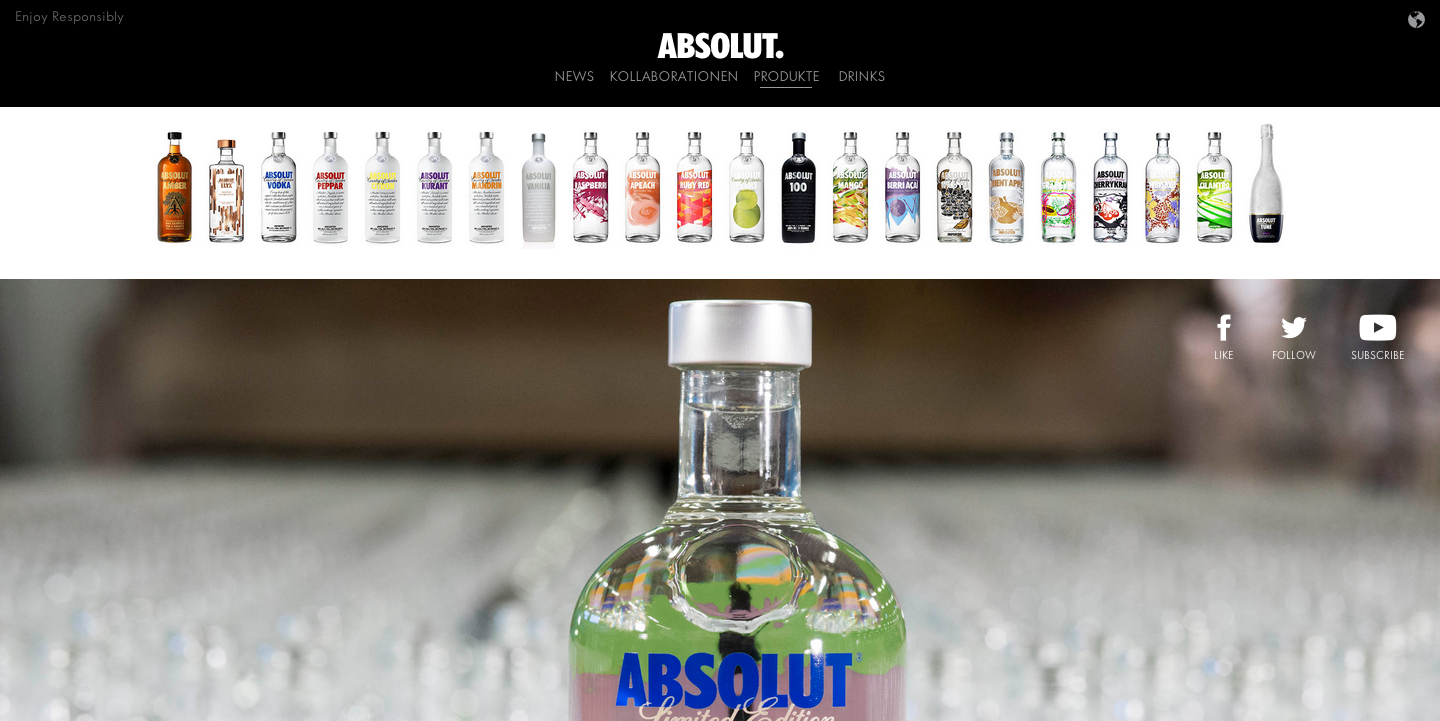
\includegraphics[scale=0.2]{bilder/absolut.png}
	\caption[Screenshot - Absolut Vodka]{Screenshot - Absolut Website}
	\label{labelname}
	\end{figure}
\end{frame}

\begin{frame}\frametitle{Beispiel Absolut II}
	\begin{tabular}{|p{2,4cm}|l|p{6cm}|}
	\hline
	  Kriterium & Punkte & Kommentar \\ \hline
  	  Aktualität & 9 & Blog mit aktuellen (nicht täglich) Einträgen; aktuelle Produktlinie \\ \hline
	  (Benutzer-) Sicherheit & 7 & Keine Speicherung Benutzerbezogener Daten; Cookies; Nutzungsverhalten wird gespeichert (Häufigkeit, Dauer...); Angeblich werden Standardschutzmaßnahmen eingesetzt \\ \hline
	  Beschreibung der Informationen & 10 & Sehr wenige Ebenen; kompakte und dennoch präzise Navigation anhand treffender Stichworte \\ \hline
 	\end{tabular}
\end{frame}

\begin{frame}\frametitle{Beispiel Absolut III}
	\begin{tabular}{|p{2,4cm}|l|p{6cm}|}
	\hline
	  Kriterium & Punkte & Kommentar \\ \hline
	  Qualität der Daten & 9 & Produkte werden sehr genau beschrieben, nicht nur im Bezug auf das Endprodukt, sondern auch Herkunft der Ausgangsmaterialien und Fertigungsprozess \\ \hline
	  UI, Erwartungshaltung, altersgerecht, etc. & 8 & Drinkrezeptsuche; UI sehr übersichtlich und intuitiv (dauernd eingeblendete Navi-Leiste oben), sowie passend für Zielgruppe; Erwartungshaltung übertroffen (Es werden Rezepte bereitgestellt... auch für anderen Alkohol, sowie ein Blog mit aktuellen Themen rund um die Marke) \\ \hline
 	\end{tabular}
\end{frame}

\begin{frame}\frametitle{Beispiel Absolut IV}
	\begin{tabular}{|p{2,4cm}|l|p{6cm}|}
	\hline
	  Kriterium & Punkte & Kommentar \\ \hline
	  Fremdsprachen & 8 & Große Mengen an Fremdsprachen; kleinere Fehler \\ \hline
	  Volltextdaten & 10 & Nahezu nur Volltextdaten; Stichwortartige Daten bei passenden Gelegenheiten (Rezepte) \\ \hline
	  Druckunter- Stützung & 0 & Nicht vorhanden \\ \hline
	  Vielfältigkeit & 10 & Hohe Vielfalt; Angebot übertrifft der einfachen Präsentation der angebotenen Produkte; Produkte werden nicht zentral abgebildet, sondern der Lifestyle von "Absolut Vodka"; Es werden Rezepte vorgeschlagen, sowie weltweite Events diskutiert \\ \hline
 	\end{tabular}
\end{frame}

\begin{frame}\frametitle{Beispiel Absolut V}
	\begin{tabular}{|p{2,4cm}|l|p{6cm}|}
	\hline
	  Kriterium & Punkte & Kommentar \\ \hline
	  Dienstleistungs- treue, Ernsthaftigkeit des Providers & 10 & Sehr durchdachtes Konzept der Informationsdarbietung, welches sicherlich mit hohem Aufwand realisiert wurde; Wirkt sehr seriös; \\ \hline
 	\end{tabular}
\end{frame}

\subsection{Negativ Beispiel}
\begin{frame}
	\frametitle{MateDrinks}
	\begin{figure}
	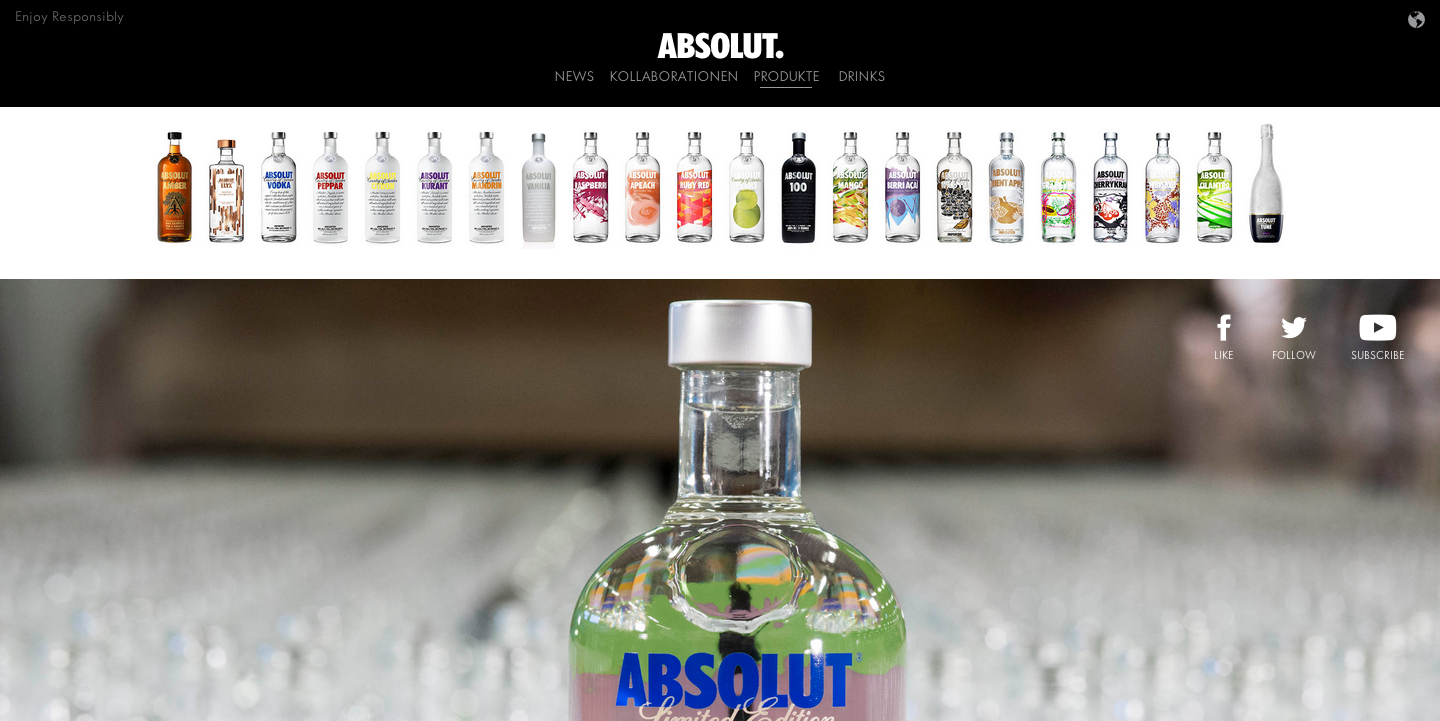
\includegraphics[scale=0.2]{bilder/absolut.png}
	\caption[Screenshot - Absolut Vodka]{Screenshot - Absolut Website}
	\label{labelname}
	\end{figure}
\end{frame}

\subsection{Fazit}
\begin{frame}
	\frametitle{Fazit}
	\begin{itemize}
		\item Bla1
		\item Bla2
		\item Bla3
	\end{itemize}
\end{frame}



\section{Datenbank-Schema}

\begin{frame}
	\frametitle{ER-Diagramm}
	\begin{figure}
	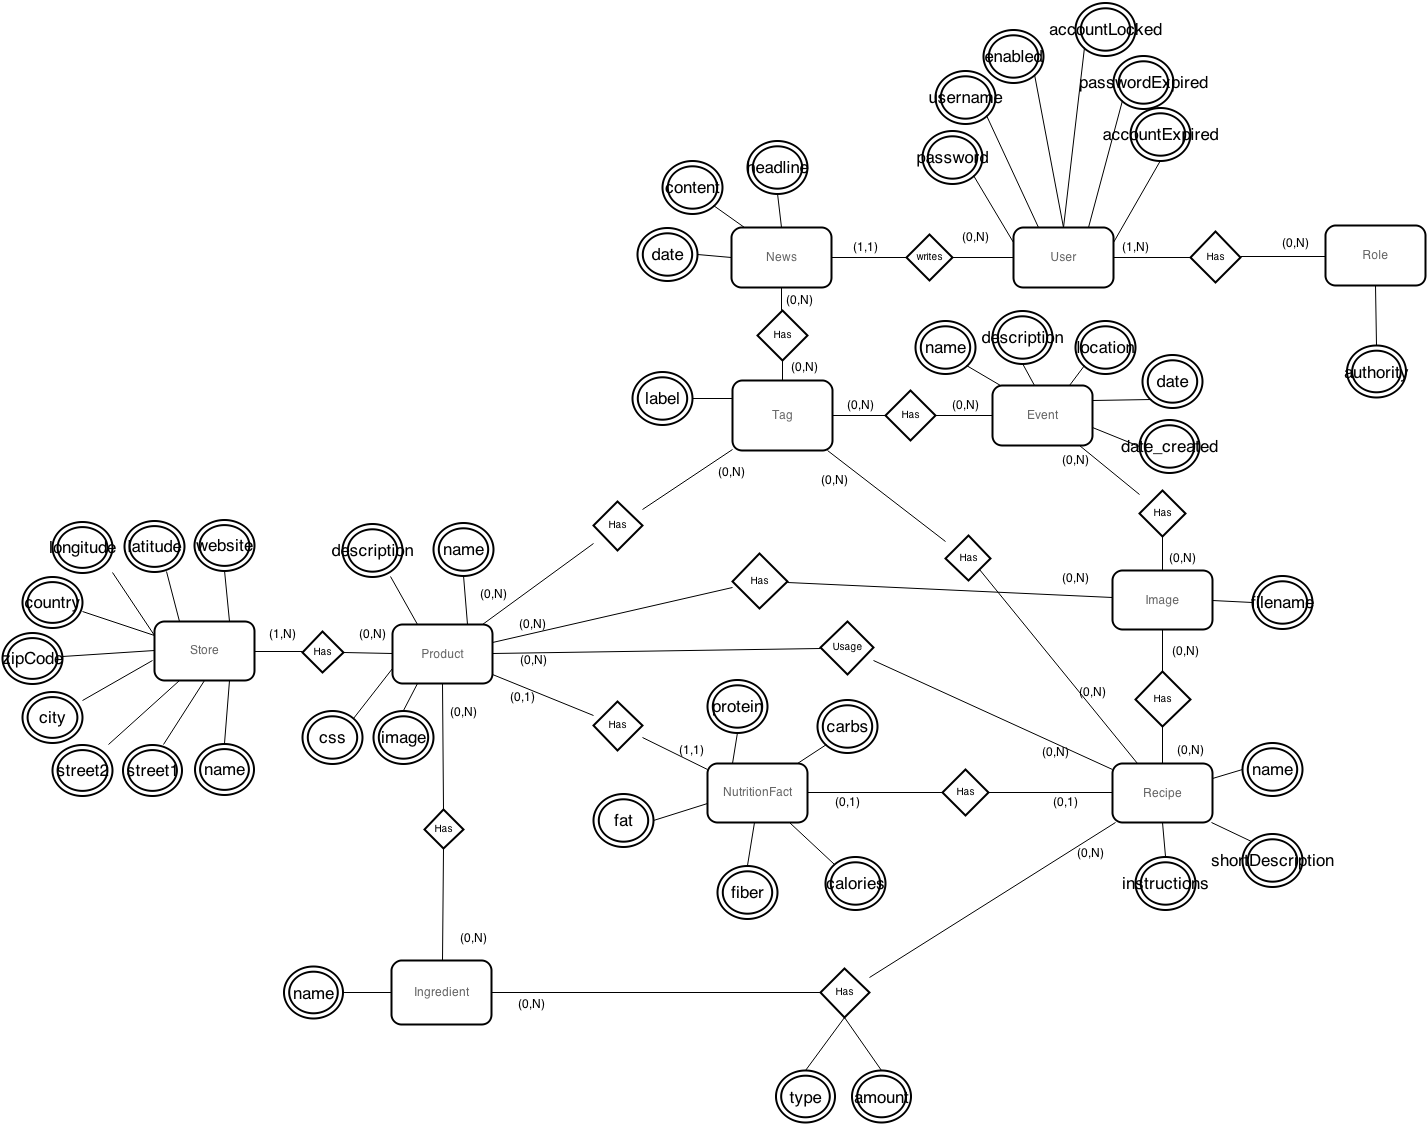
\includegraphics[scale=0.2]{bilder/er-diagramm.png}
	\end{figure}
\end{frame}

\begin{frame}
	\frametitle{Story}
	\begin{figure}
	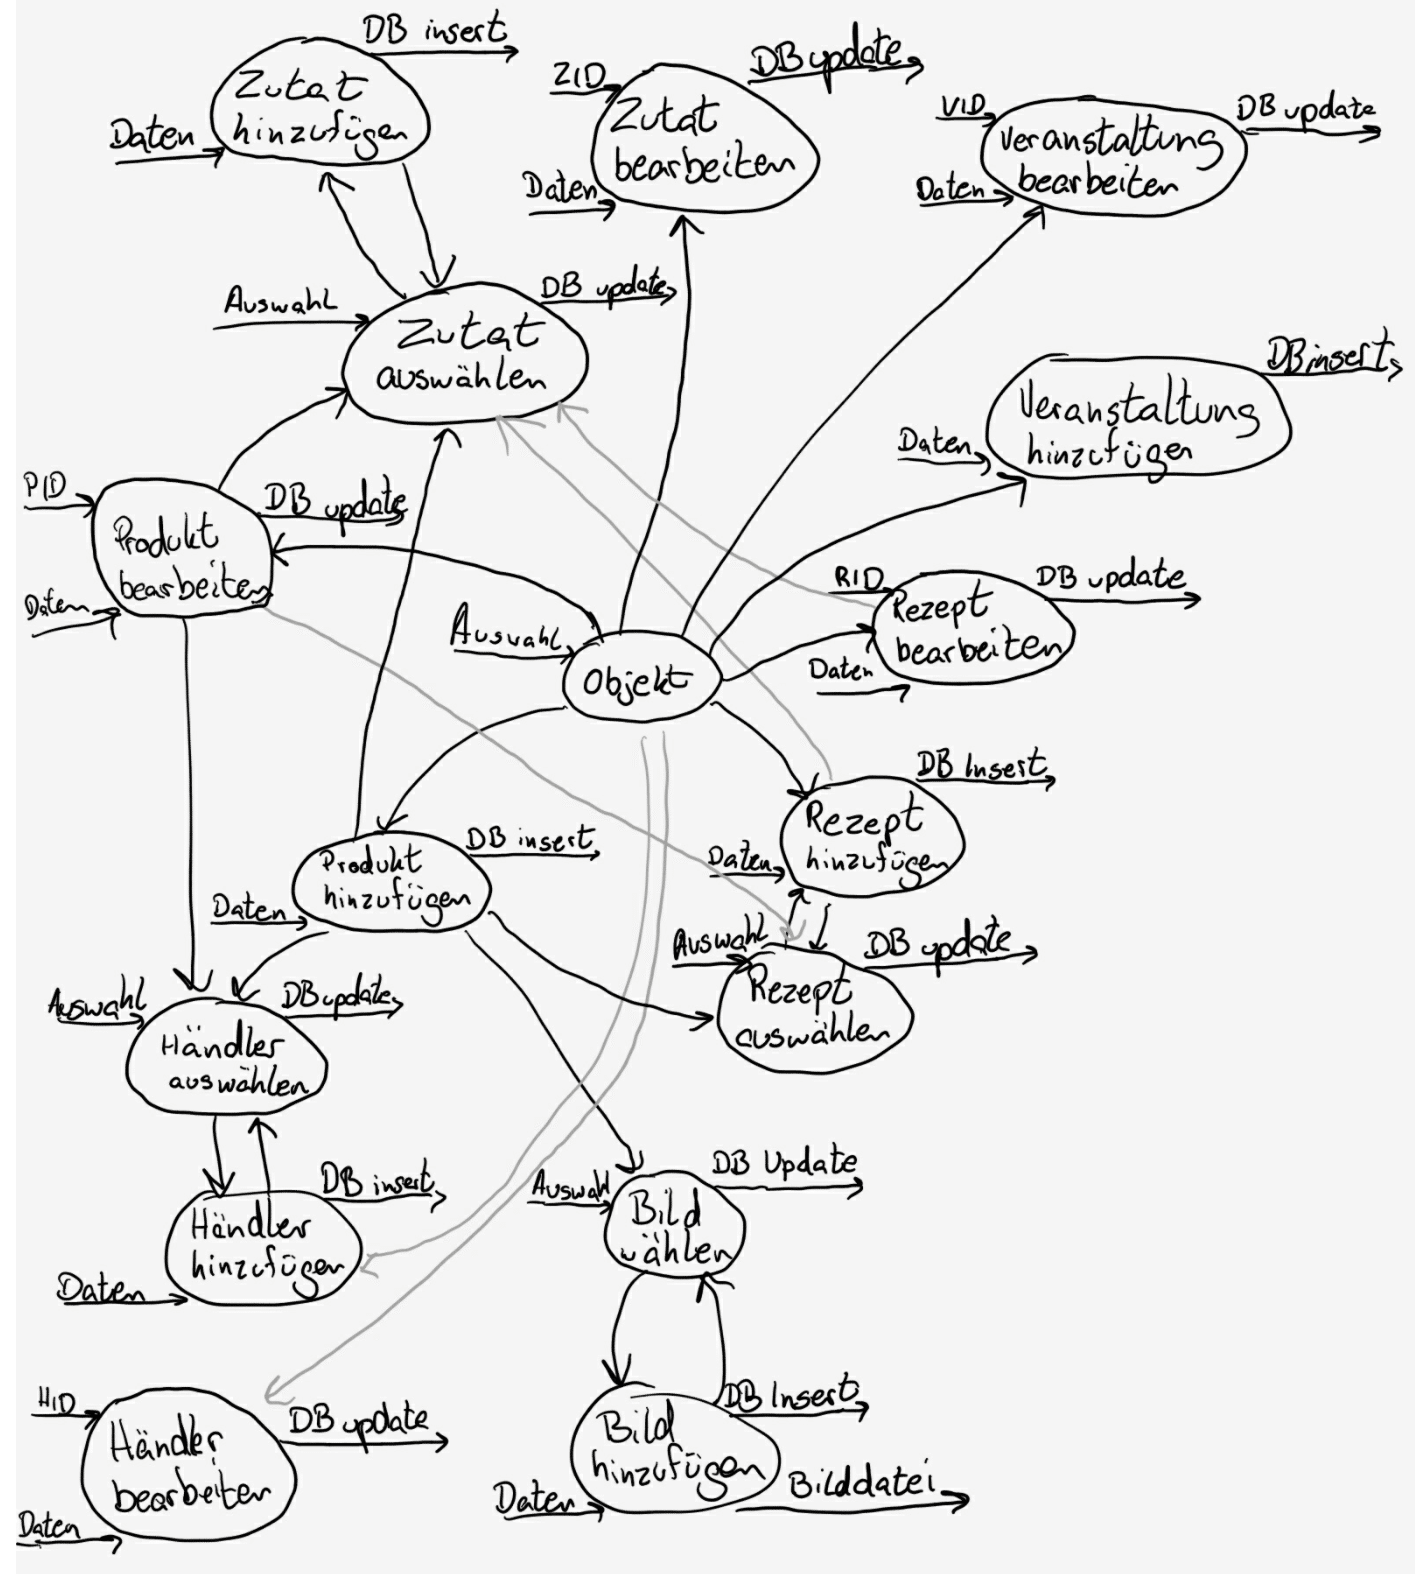
\includegraphics[scale=0.125]{bilder/bubble.png}
	\end{figure}
\end{frame}

\section{Live-Demo} 
\begin{frame}
	\frametitle{Demonstration} 
	Behold the pure beauty of our creation!
\end{frame}

\section{Bildverzeichnis}
\begin{frame}
	\listoffigures
	%Rausnehmen, wenns nicht geht
\end{frame}

\end{document}